\chapter{Caso de uso}
\label{caso_de_uso}

En este capítulo presentaremos el problema elegido como caso de uso para nuestra implementación, así como la justificación de por qué se ha elegido este problema y por qué es adecuado para el algoritmo implementado. Por último se hablarán de las limitaciones y el ámbito de uso del algoritmo.\\


\section{Descripción del problema}
\label{problema}

El problema seleccionado para el caso de uso han sido las competeticiones de robótica. Esta decisión está justificada por la gran variedad de retos de distinto carácter que presentan estas competiciones, así como la naturaleza práctica de las mismas.\\

Concretamente, la implementación realizada se basa en una aplicación típica de robots rastreadores de competición. En estas competiciones, los robots han pasan por diferentes pruebas, como encontrar la salida de un laberinto o cruzar un escenario con obtáculos. En la figura \ref{fig:competi1}, puede observarse cómo estos obstáculos generalmente no tienen texturas y utilizan formas muy básicas. Con esto se intenta abstraer al robot de perturbaciones físicas y visuales, presentando un entorno modular y simple.\\

\begin{figure}[h]
		\centering
        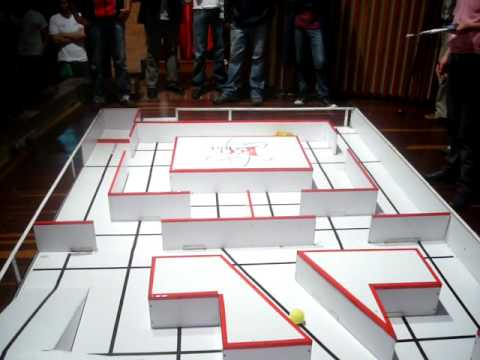
\includegraphics[width=0.5\textwidth]{images/competi1.jpg}
        \caption{Escenario de competición robótica}
        \label{fig:competi1}
\end{figure}  

La simplicidad en el aspecto y forma de los obstáculos, así como el hecho de que estos obstáculos son modulares permite simular una gran cantidad de situaciones y escenarios distintos de navegación, siendo muy fácil reconfigurar su posición y unir obstáculos para crear obstáculos más complejos.\\

Siguiendo el modelo de algunas competiciones existentes se han desarrollado tres escenarios diferentes, de distinto nivel del dificultad, cada uno con características exclusivas a ese escenario. Se ha procurado también que estos escenarios fuesen similares a los presentados por los autores del artículo seleccionado, de forma que se pudiese llevar a cabo una comparación entre los resultados obtenidos con nuestra implementación y los presentados en el artículo original. Como se ha mencionado anteriormente, la competición emulada en este trabajo es la de robots rastreadores, y por tanto la forma y disposición de los obstáculos se asemejará en la medida de lo posible a la propia de este tipo de competiciones.\\

Al tratarse de una competición, se ha tenido en cuenta el tiempo empleado por el robot para la planificación del camino a seguir, así como el tiempo dedicado por el robot para el desplazamiento del mismo desde el origen hasta la meta.\\

Por último, los alumnos han elegido este caso de uso debido a la posibilidad real de presentar un robot de competición con estos algoritmos de planificación a un concurso real, dependiendo de los resultados obtenidos en las pruebas realizadas en simulación. No obstante, esta parte del desarrollo se pretende realizar como trabajo futuro y, por tanto, no ha sido realizada como parte de este trabajo.\\


\section{Selección del algoritmo}
\label{justificacion}

El algoritmo seleccionado para realizar el caso de uso ha sido el presentado en el artículo complementario, \textit{Quasi-randomized Probabilistic Roadmaps (Q-PRMs)}.\\

En este caso la elección ha sido llevada a cabo por motivos ajenos a nuestras personas, ya que el artículo principal no ofrecía un algoritmo de planificación, sino que realizaba una crítica o anotación puntual a aspectos muy concretos de un tercer artículo escrito por Rodney Brooks. Al tratarse de detalles muy dependientes del mencionado artículo, y dado que nuestros compañeros se encontraban realizando su trabajo sobre dicho artículo, hemos optado por realizar la implementación del algoritmo presentado en el artículo complementario. De esta forma conseguimos una mayor variedad de algoritmos en los trabajos de la asignatura, así como la posibilidad de comparar el algoritmo Q-PRM estudiado en este trabajo con el algoritmo de representación del espacio libre como conos generalizados de nuestros compañeros.\\

Además, la naturaleza probabilística y, según los autores, más rápida computacionalmente de los algoritmos basados en PRM, y que por tanto incluyen al Q-PRM hacen de estos algoritmos una elección interesante a evaluar para competiciones de robots, en las que suele primar el tiempo como uno de los factores decisivos a la hora de puntuar en las pruebas.\\


\section{Ámbito de uso}
\label{ambito}

En la opinión de los alumnos, este algoritmo se ajusta adecuadamente al caso de uso propuesto, y por tanto es realista.\\

No obstante, si se quisiera implementar este algoritmo en un robot de competición real se debería comprobar que la capacidad de cómputo requerida para llevar a cabo la planificación mediante el uso de Q-PRMs puede ser satisfecha por el hardware del robot de competición.\\

También sería necesario comprobar que el tiempo de ejecución del algoritmo no se ve incrementado en exceso al ser ejecutado en el hardware del robot de competición, que se supone más limitado que los ordenadores de sobremesa utilizados por los alumnos para las pruebas e implementación del algoritmo.\\

Por último, para que este método pudiese ser aplicado satisfactoriamente, el robot debería disponer del mapa del entorno en el momento de realizar la planificación. Este plano podría ser suministrado por los organizadores, obtenido por los participantes mediante medidas del terreno o computado por el robot de competición mediante técnicas de mapeado o SLAM (Simultaneous Location and Mapping).\\

De tenerse en cuenta todas estas limitaciones potenciales, los alumnos creen que ese algoritmo podría ser empeado de forma realista y competitiva en pruebas similares a las usadas como demostración en este trabajo.